\section{Summary}

\begin{frame}{Summary}
This work brings to HoTT
\begin{itemize}
\item connections, curvature, and vector fields
\item the index of a vector field
\item a theorem in dimension 2 that total curvature = total index
\end{itemize}
\end{frame}

\begin{frame}{Classical \( \to \) HoTT}
Let \( M \) be a smooth, oriented 2-manifold without boundary, \( F_A \) the curvature of a connection \( A \) on the tangent bundle, and \( X \) a vector field with isolated zeroes \( x_1,\ldots,x_n \).
% https://q.uiver.app/#q=WzAsNSxbMCwwLCJcXGRpc3BsYXlzdHlsZXtcXGZyYWN7MX17MlxccGl9XFxpbnRfTSBGX0F9Il0sWzEsMCwiXFxkaXNwbGF5c3R5bGV7XFxzdW1fe2k9MX1ebiBcXG1hdGhybXtpbmRleH1fWCh4X2kpfSJdLFswLDEsIlxcZGlzcGxheXN0eWxle1xcT21lZ2FcXGxlZnQoXFxzdW1fe1xcbWF0aHJte2ZhY2VzfVxcIGZ9XFxmbGF0X2ZcXHJpZ2h0KX0iXSxbMSwxLCJcXGRpc3BsYXlzdHlsZXtcXHN1bV97XFxtYXRocm17ZmFjZXN9fUleWF9mfSJdLFsyLDAsIlxcY2hpKE0pIl0sWzAsMSwiIiwwLHsibGV2ZWwiOjIsInN0eWxlIjp7ImhlYWQiOnsibmFtZSI6Im5vbmUifX19XSxbMCwyXSxbMSwzXSxbMiwzLCIiLDIseyJsZXZlbCI6Miwic3R5bGUiOnsiaGVhZCI6eyJuYW1lIjoibm9uZSJ9fX1dLFsxLDQsIiIsMix7ImxldmVsIjoyLCJzdHlsZSI6eyJoZWFkIjp7Im5hbWUiOiJub25lIn19fV1d
\[\begin{tikzcd}[ampersand replacement=\&,column sep=tiny]
  {\displaystyle{\frac{1}{2\pi}\int_M F_A}} \& {\displaystyle{\sum_{i=1}^n \mathrm{index}_X(x_i)}} \& {\chi(M)} \\
  {\displaystyle{\sum_{\mathrm{faces}\ F}\flat_F}} \& {\displaystyle{\sum_{\mathrm{faces}\ F}L^X_F}}
  \arrow[equals, from=1-1, to=1-2]
  \arrow[from=1-1, to=2-1]
  \arrow[equals, from=1-2, to=1-3]
  \arrow[from=1-2, to=2-2]
  \arrow[equals, from=2-1, to=2-2]
\end{tikzcd}\]
\end{frame}

\begin{frame}{Classical index}
Near an isolated zero there are only three possibilities: index 0, 1, --1.

Index is the winding number of the field as you move clockwise around the zero.
\begingroup
\colorlet{veccol}{cmu_red}
\colorlet{myblue}{blue!60!black}
\tikzstyle{vector}=[->,thick,veccol,style={-{Stealth[scale=0.9]}}]
\pgfmathsetmacro{\R}{1}%
\pgfmathsetmacro{\r}{0.03}%
\pgfmathsetmacro{\N}{8}%
\pgfmathsetmacro{\ang}{60}%
\pgfmathsetmacro{\RR}{0.5}%
\[
% zero
\begin{tikzpicture}
  \fill[myblue] (0,0) circle (\r);
  \foreach \x/\y in {-1/0,-1/1,0/1,1/1,1/0,-1/-1,0/-1,1/-1}{
    \draw[vector] (\x*0.5*\R,\y*0.5*\R) ++ (\ang-180:\R/2) --++ (\ang:\R);
  }
  \node at (0,-1.35*\R) {index 0};
\end{tikzpicture}\,\,
% outward
\begin{tikzpicture}
  \fill[myblue] (0,0) circle (\r);
  \foreach \i [evaluate={\ang=\i*360/\N;}] in {0,...,\N}{
    \draw[vector] (\ang:0.1*\R) --++ (\ang:\R);
  }
  \node at (0,-1.35*\R) {index +1};
\end{tikzpicture}\,\,
% inward
\begin{tikzpicture}
  \fill[myblue] (0,0) circle (\r);
  \foreach \i [evaluate={\ang=\i*360/\N;}] in {0,...,\N}{
    \draw[vector] (\ang:1.1*\R) -- (\ang:0.1*\R);
  }
  \node at (0,-1.35*\R) {index +1};
\end{tikzpicture}\,\,
% counterclock
\begin{tikzpicture}
  \fill[myblue] (0,0) circle (\r);
  \foreach \R in {0.44,0.88}{
    \foreach \i [evaluate={\ang=\i*360/\N;}] in {1,...,\N}{
      \draw[vector] (\ang:\R) --++ (\ang+90:\RR);
    }
  }
  \node at (0,-1.3*\R) {index +1};
\end{tikzpicture}\,\,
% clockwise
\begin{tikzpicture}
  \fill[myblue] (0,0) circle (\r);
  \foreach \R in {0.44,0.88}{
    \foreach \i [evaluate={\ang=\i*360/\N;}] in {1,...,\N}{
      \draw[vector] (\ang:\R) --++ (\ang-90:\RR);
    }
  }
  \node at (0,-1.3*\R) {index +1};
\end{tikzpicture}\,\,
% minus one
\pgfmathsetmacro{\r}{0.03}%
\pgfmathsetmacro{\N}{20}%
\pgfmathsetmacro{\ang}{10}%
\begin{tikzpicture}
  \fill[myblue] (0,0) circle (\r);
  \foreach \R in {0.88}{
    \foreach \i [evaluate={\ang=\i*360/\N;}] in {1,...,\N}{
      \draw[vector] (\ang:\R) --++ (-\ang-90:\RR);
    }
  }
  \node at (0,-1.3*\R) {index --1};
\end{tikzpicture}

\]
\endgroup
% \includegraphics[width=420pt]{figs/needham_indexes.pdf}
\end{frame}

\begin{frame}{Poincaré-Hopf theorem}
The total index of a vector field is the Euler characteristic.

Examples:
\vspace{3ex}
\begin{columns}
\begin{column}{0.5\textwidth}
\centering
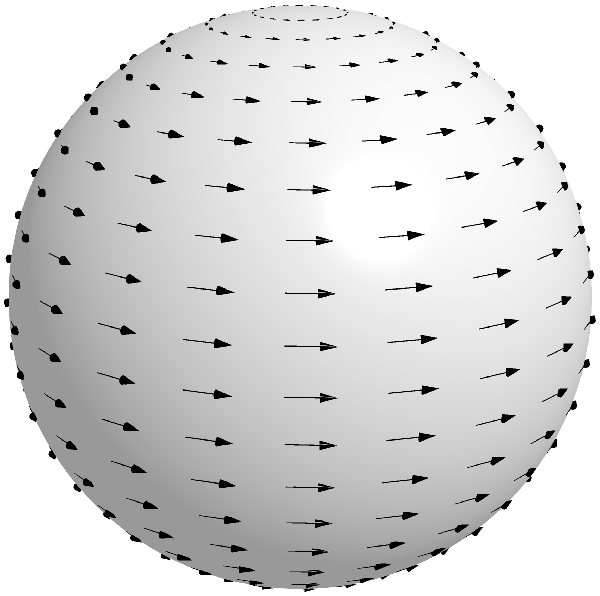
\includegraphics[width=20ex]{figs/sphere_vf_rotate.pdf}

Rotation: index +1 at each pole = \textbf{2}
\end{column}

\begin{column}{0.5\textwidth}
\centering
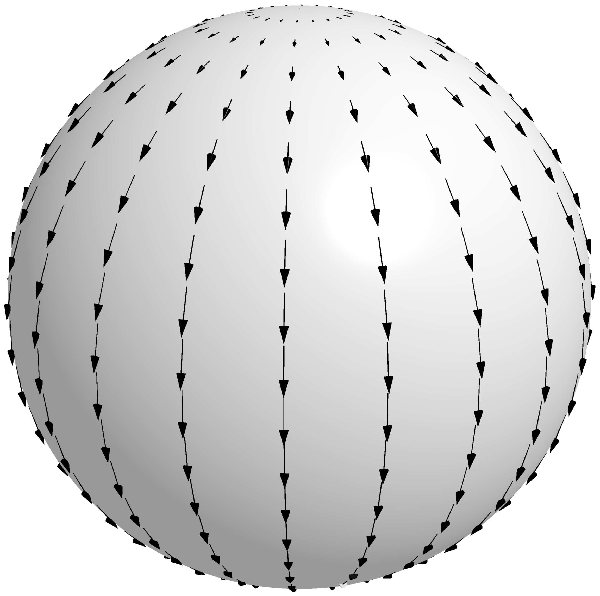
\includegraphics[width=20ex]{figs/sphere_vf_morse.pdf}

Height: index +1 at each pole = \textbf{2}
\end{column}
\end{columns}
\end{frame}

\begin{frame}{Gauss-Bonnet theorem}
Total curvature divided by \( 2\pi \) is the Euler characteristic.

Curvature in 2D is a function \( F_A:M\to \rr \).

\( \int_M F_A \) sums the values at every point. 
\begin{columns}
\begin{column}{0.58\textwidth}
\centering
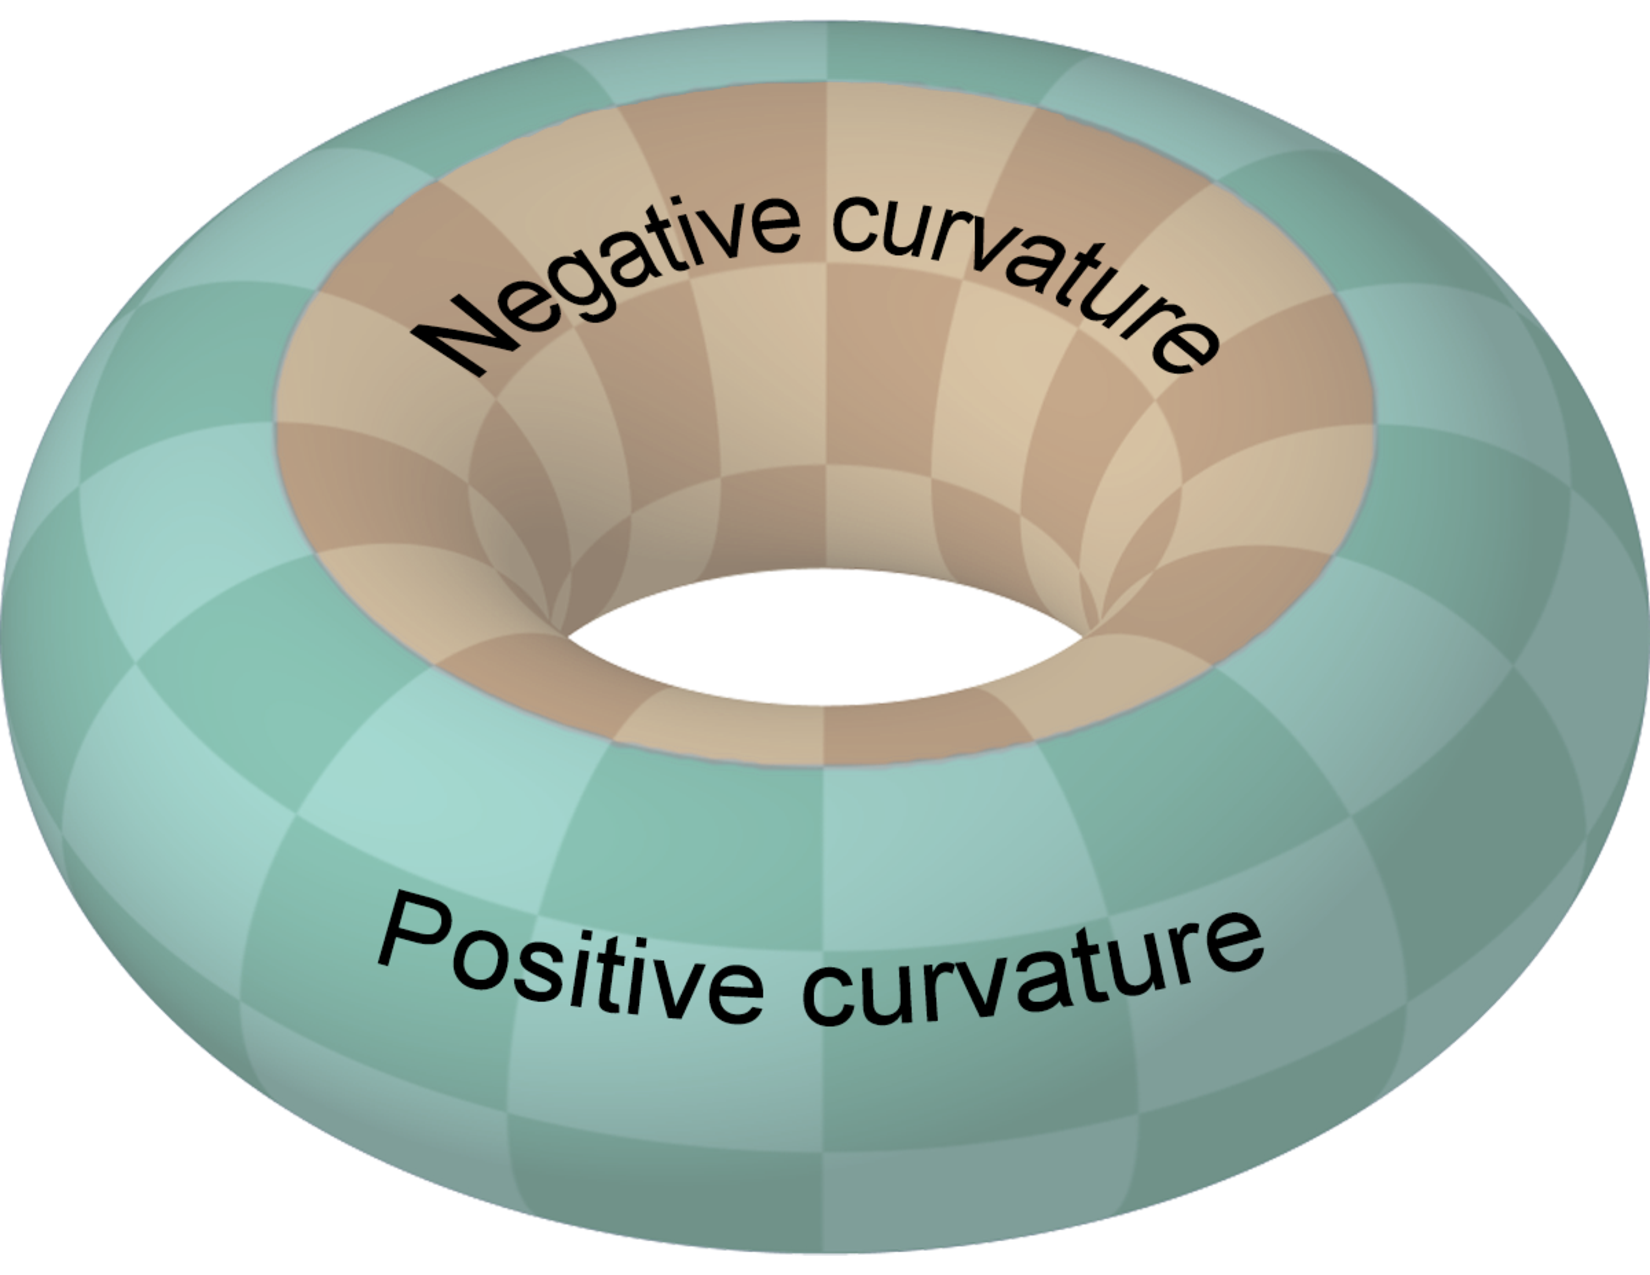
\includegraphics[height=20ex]{figs/torus_gauss_bonnet.pdf}

Positive and negative curvature cancel: \textbf{0}
\end{column}
\begin{column}{0.42\textwidth}
\centering
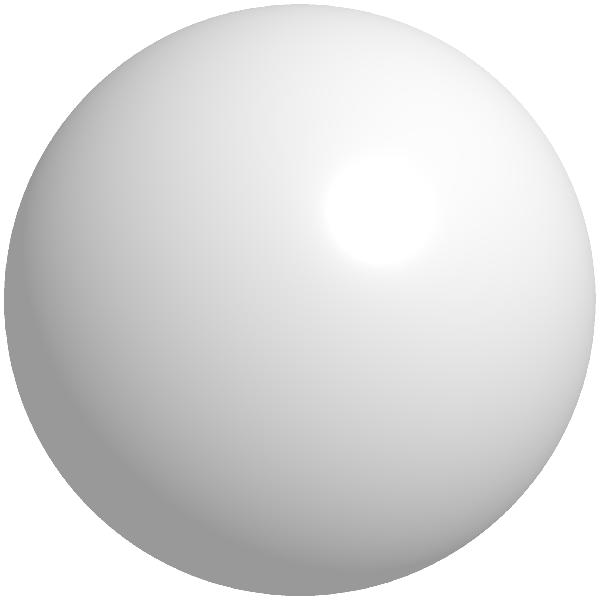
\includegraphics[height=20ex]{figs/sphere_curvature.pdf}

Constant curvature 1, area \( 4\pi \): \textbf{2}
\end{column}
\end{columns}
\end{frame}

\begin{frame}{Plan}
\begin{itemize}
\item Combinatorial manifolds
\item Torsors and classifying maps
\item Connections and curvature
\item Vector fields
\item Main theorem
\end{itemize}
\end{frame}

\begin{frame}{HoTT background}
\begin{enumerate}
\item \alert{Symmetry},\\
Bezem,~M., Buchholtz,~U., Cagne,~P., Dundas,~B.~I., and Grayson,~D.~R., (2021-) \\
\url{https://github.com/UniMath/SymmetryBook}.

\item \alert{Central H-spaces and banded types},\\
Buchholtz,~U., Christensen,~J.~D. , Flaten,~J.~G.~T., and Rijke,~E. (2023) \\
arXiv:2301.02636

\item \alert{Nilpotent types and fracture squares in homotopy type theory},\\
Scoccola,~L. (2020) \\
MSCS 30(5). arXiv:1903.03245
\end{enumerate}
\end{frame}

